The diagram shows the deployment of the system and its structure.

\begin{figure}[H]
	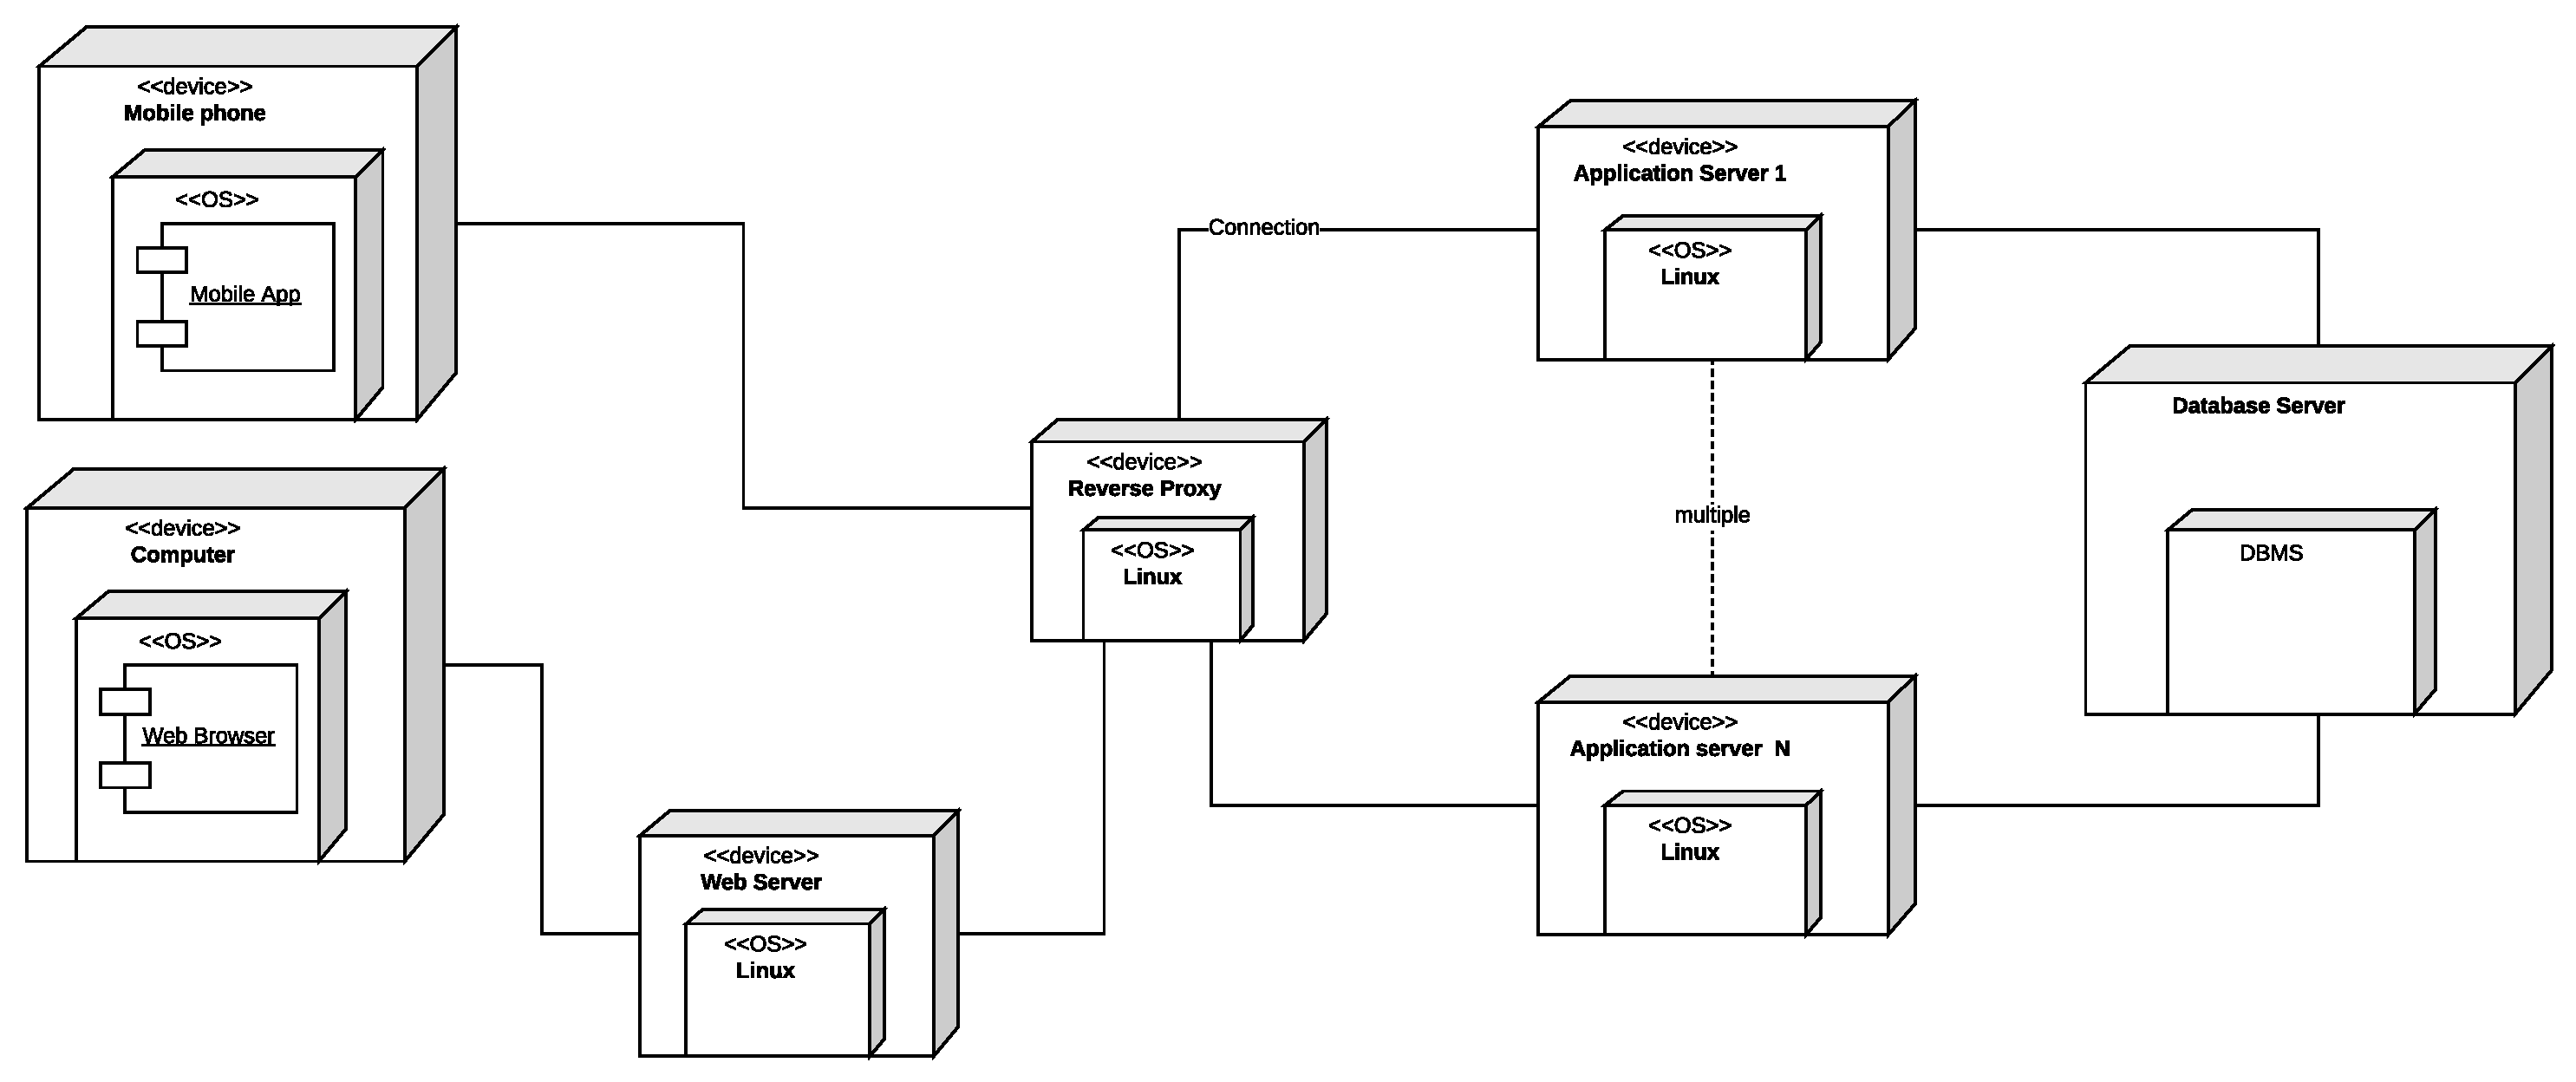
\includegraphics[width=\textwidth,height=\textheight,keepaspectratio]{assets/DeploymentDiagram.pdf}
	\caption{Deployment diagram}
	\label{fig:DD}
\end{figure}

\begin{itemize}
    \item \textbf{Client}: represents the first layer. We distinguish between 2 typologies of clients: Web Browser and Mobile app.
    \item \textbf{Server}: is part of the second layer. 
    We distinguish:
    \begin{itemize}
        \item Application server: contains all the business logic of the system.
        \item Web Server: contains the data concerning to the web pages
    \end{itemize}
    \item \textbf{Reverse proxy}: is part of the second layer of the system.
    Is a type of proxy server that retrieves resources on behalf of a client from one or more servers.
    \item \textbf{Database}: is the third layer of the system that stores all the data. 
    The system uses a relational DBMS.
\end{itemize}
